\documentclass[a4paper]{article}
% Kodowanie latain 2
%\usepackage[latin2]{inputenc}
\usepackage[T1]{fontenc}
% Można też użyć UTF-8
\usepackage[utf8]{inputenc}

% Język
\usepackage[polish]{babel}
% \usepackage[english]{babel}

% Rózne przydatne paczki:
% - znaczki matematyczne
%\usepackage{amssymb}
\usepackage{amsmath, amsfonts}
% - wcięcie na początku pierwszego akapitu
\usepackage{indentfirst}
% - komenda \url 
\usepackage{hyperref}
% - dołączanie obrazków
\usepackage{graphicx}
% - szersza strona
\usepackage[nofoot,hdivide={2cm,*,2cm},vdivide={2cm,*,2cm}]{geometry}
\usepackage{lmodern}
\usepackage{changepage}
\usepackage{pythonhighlight}
\frenchspacing
\title{\emph{Sprawozdanie z zadania egzaminacyjnego nr 1}}
\author{Piotr Piesiak}
\begin{document}
\maketitle
\section{Rozkład normalny}
Rozkład normalny możemy bardzo często zaobserwować w naturze. W statystyce używamy go do opisu wielu obserwacji takich jak inteligencja, wzrost, czy natężenie źródła światła, przez co jest jednym z najważniejszych rozkładów prawdopodobieństwa. Gęśtość rozkładu normalnego przyjmuje dwa parametry ($X \sim N(\mu,\sigma^2)$):
\begin{enumerate}
\item $\mu$ - oznaczające średnią
\item $\sigma^2$ - oznaczające wariancję, $\sigma$ jest odchyleniem standardowym
\end{enumerate}
i określa się wzorem
$$f(x) = \frac{1}{\sigma\sqrt{2\cdot\pi}}\,\exp\left(\frac {-(x-\mu )^2} {2\sigma^2}\right) ,\,x \in \mathbb{R}$$
\begin{figure}[htbp]
\centerline{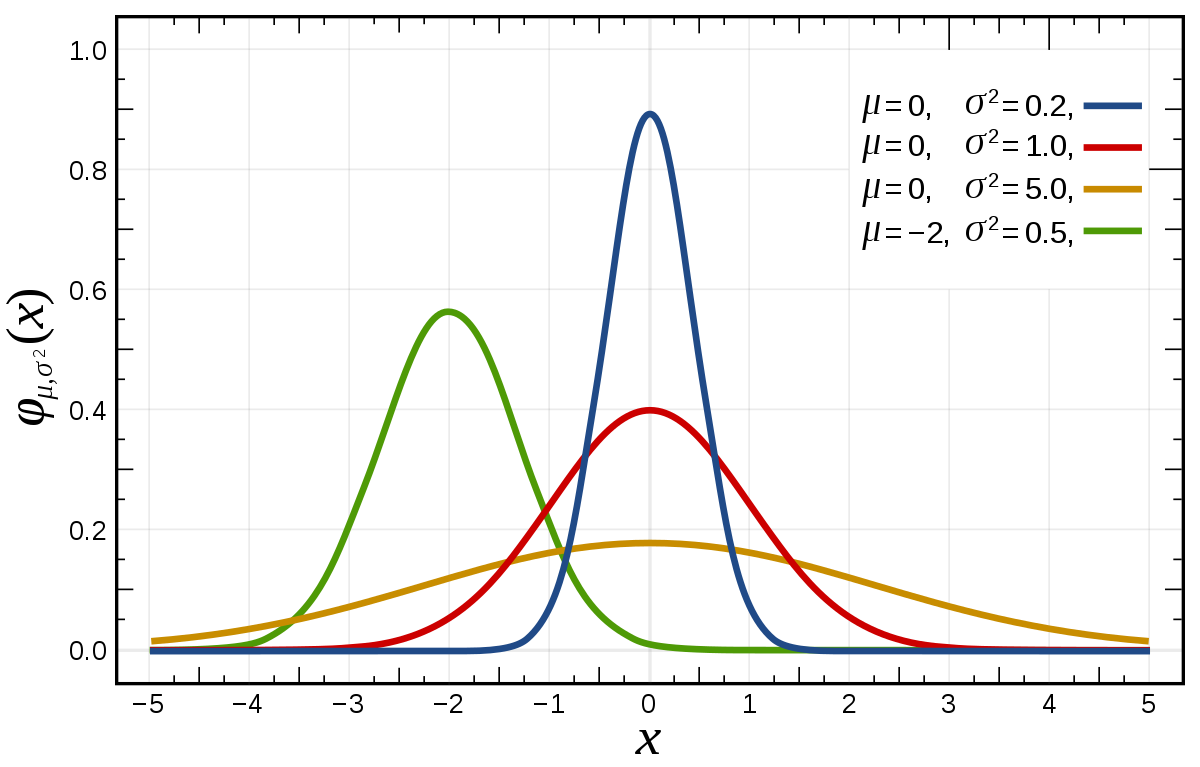
\includegraphics[scale=.15]{wykres_ND.png}}
\caption{wykres gęstości prawdopodobieństwa rozkładu normalnego dla różnych parametrów \newline(źródło: wikipedia/Rozkład\_normalny)}
\label{fig:ND}
\end{figure}
\subsection{Standardowy rozkład normalny}
Standardowy rozkład normalny jest szczególnym przypadkiem rozkładu normalnego dla $\mu = 0$ oraz $\sigma^2 = 1$, ma gęstość określoną wzorem:
$$f(x) = \frac{1}{\sqrt{2\cdot\pi}}\exp\left(-\frac{x^2}{2}\right) ,\, x \in \mathbb{R}$$
W tym zadaniu zajmiemy się obliczeniem dystrybuanty standardowego rozkładu normalnego, czyli wartości funkcji:
$$\Phi(t) = \int\limits_{-\infty}^t f(x)\,dx = \int\limits_{-\infty}^t \frac{1}{\sqrt{2\cdot\pi}}\,\exp\left(-\frac{x^2}{2}\right)\,dx,\, t \in \mathbb{R}$$
\section{Obliczenie funkcji dystrybuanty}
Niestety, pomimo że wiemy:
$$\int\limits_{-\infty}^{\infty} \exp(-x^2)\,dx = \sqrt{\pi}$$ to całki oznaczonej z $\exp(-x^2) $ nie da się obliczyć dokładnie metodą analityczną i jesteśmy zmuszeni do korzystania z przybliżeń pochodzących z tablic (dostępnych w internecie) lub własnego programu przybliżającego całkę. My skorzystamy z własnego programu, spróbujmy więc ułatwić zadanie komputerowi i pozbyć się granicy $\-inf$ w liczeniu całki.
\subsection{Symetryczność funkcji gęstości}
Zauważmy, że funkcja gęstości rozkładu normalnego jest symetryczna. Łatwo to zaobserwować na wykresie (rys. ~\ref{fig:ND}), lub też wywnioskować ze wzoru funkcji:
$$f(x) = \frac{1}{\sqrt{2\cdot\pi}}\exp\left(-\frac{x^2}{2}\right) = \frac{1}{\sqrt{2\cdot\pi}}\exp\left(-\frac{(-x)^2}{2}\right) = f(-x)$$
Korzystając zatem z symetryczności funkcji gęstości (f) możemy zapisać:
$$\Phi(t) = \int\limits_{-\infty}^t f(x)\,dx = 2 \cdot \int\limits_{0}^t f(x)\,dx = 2 \cdot \int\limits_{0}^t \frac{1}{\sqrt{2\cdot\pi}}\,\exp\left(-\frac{x^2}{2}\right)\,dx $$
\subsection{Przekształcenie funkcji dystrybuanty}
Skorzystajmy teraz z własności funkcji gęstości, a mianowicie:
$$\int\limits_{-\infty}^{\infty} f(x)\,dx = 1$$
korzystając z obserwacji 2.1:
$$\int\limits_{-\infty}^{\infty} f(x)\,dx = 2 \cdot \int\limits_{0}^{\infty} f(x)\,dx =1$$
czyli
$$\int\limits_{-\infty}^{0} f(x)\,dx = \int\limits_{0}^{\infty} f(x)\,dx = \frac{1}{2}$$
Po tych kilku prostych obserwacjach wróćmy do naszego problemu obliczania dystrybuanty:
$$\Phi(t) = \int\limits_{-\infty}^t f(x)\,dx = \int\limits_{-\infty}^t \frac{1}{\sqrt{2\cdot\pi}}\,\exp\left(-\frac{x^2}{2}\right)\,dx,\, t \in \mathbb{R}$$

Rozpatrzmy dwa przypadki:
\begin{enumerate}
\item $t \geq 0$
$$\Phi(t) = \int\limits_{-\infty}^0 f(x)\,dx \,+ \int\limits_{0}^t f(x)\,dx = \int\limits_{-\infty}^0 \frac{1}{\sqrt{2\cdot\pi}}\,\exp\left(-\frac{x^2}{2}\right)\,dx \newline \,+ \int\limits_{0}^t \frac{1}{\sqrt{2\cdot\pi}}\,\exp\left(-\frac{x^2}{2}\right)\,dx$$
czyli:
$$\Phi(t) = \frac{1}{2} + \frac{1}{\sqrt{2\cdot\pi}} \cdot \int\limits_{0}^t \exp\left(-\frac{x^2}{2}\right)\,dx$$
\item $t < 0$
\\ Skorzystajmy jeszcze raz z symetryczności funkcji gęstości:
$$\int\limits_{-\infty}^t f(x)\,dx \stackrel{\text{t < 0}}{=}
 \int\limits_{-t}^{\infty} f(x)\,dx $$
 $$\frac{1}{2} = \int\limits_{0}^{\infty} f(x)\,dx = \int\limits_{0}^{-t} f(x)\,dx \, + \int\limits_{-t}^{\infty} f(x)\,dx$$
 czyli wzór na dystrybuantę wygląda:
 $$\Phi(t) = \frac{1}{2} - \int\limits_{0}^{-t} f(x)\,dx = \frac{1}{2} - \frac{1}{\sqrt{2\cdot\pi}} \cdot \int\limits_{0}^{-t} \exp\left(-\frac{x^2}{2}\right)\,dx$$
\end{enumerate}
Zauważmy, że po przekształceniu w oby przypadkach problem obliczenia dystrybuanty sprowadza się do obliczenia wartości całki $I(a)$:
$$I(a) = \int\limits_{0}^{a} \exp\left(-\frac{x^2}{2}\right)\,dx $$
\subsection{Szkic algorytmu obliczającego dystrybuantę}
Zakładając, że potrafimy obliczyć całkę $I(a)$ możemy skonstruować algorytm, który obliczałby dystrybuantę:
\begin{python}
import math
def phi(t):
	if t >= 0:
		return 1/2 + 1/(math.sqrt(2 * math.pi)) * I(t)
	else:
		return 1/2 - 1/(math.sqrt(2 * math.pi)) * I(-t)
\end{python}
\section{Metody całkowania numerycznego}
\subsection{Metoda złożonych trapezów}
W metodzie dej dzielimy przedział całkowania (bardzo intuicyjnie) $(n+1)$ równoodległymi punktami na podprzedziały:
$$a = x_0 < x_1 < x_2 < x_3 < \ldots < x_{n-1} < b = x_n$$
i pole pod wykresem między punktami $x_i, x_{i+1}$ przybliżamy polem trapezu tzn. $\frac{(f(x_{i}) + f(x_{i+1})) \cdot (x_{i+1} - x_i)}{2}$ (rys. ~\ref{fig:trapez})
\begin{figure}[htbp]{}
\centerline{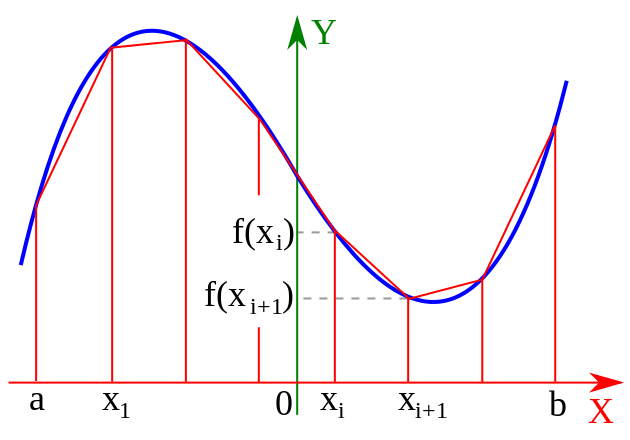
\includegraphics[scale=.4]{wykres_trapez.png}}
\caption{Zobrazowanie działania metody (źródło: wikipedia/Wzór\_trapezów)}
\label{fig:trapez}
\end{figure}

Ostatecznie otrzymujemy wzór:
$$\int\limits_{a}^{b} f(x)\,dx \approx \sum_{i = 0}^{n - 1}\frac{(f(x_{i}) + f(x_{i+1})) \cdot (x_{i+1} - x_i)}{2} = \sum_{i = 0}^{n - 1}\frac{(f(x_{i}) + f(x_{i+1})) \cdot (\frac{b - a}{n})}{2} = $$
$$= \frac{b - a}{2\cdot n} \cdot (f(a) + 2\cdot f(x_1) + 2\cdot f(x_2) + \ldots 2 \cdot f(x_{n-1}) + f(b)))$$
Prosta implementacja tej metody wygląda:
\begin{python}
def compositeTrapezoid(n,a,b):
    h = (b-a)/n
    sum = 0
    for i in range(1,n):
        sum += f(a + i*h)
    return (1/2)*h*(f(a) + 2*sum + f(b))
\end{python}
\subsection{Metoda Romberga}
W tej metodzie dzielimy przedział całkowania $(a,b)$na $2^n$ równych części:
$$a = x_0 < x_1 < x_2 < x_3 < \ldots < x_{2^n-1} < b = x_{2^n}$$
Niech $T(n)$ oznacza wynik złożonego wzoru trapezów dla n przedziałów. Możemy przedstawić metodę Romberga rekurencyjnie:
$$
\begin{cases}
R_{0,i} &: T(2^n)\\ 
\ R_{m,i} &: \frac{4^m\cdot R_{m-1,i+1}-R_{m-1,i}}{4^m-1}
\end{cases}
$$
Sprowadza się to do obliczenia współczynników tablicy Romberga, czyli wyznaczenia rekurencyjnie kolejnych kolum. Otrzymamy w ten sposób coraz lepsze przybliżenie funkcji: \\
$R_{0,0}$ \\
$R_{0,1}$$R_{1,0}$ \\
$R_{0,2}$$R_{1,1}$$R_{2,0}$ \\
$R_{0,3}$$R_{1,2}$$R_{2,1}$$R_{3,0}$\\
$\ldots$ \\
Implementacja wykorzystująca tę rekurencję wyglada następująco: (procedura RombergsMethod zwraca kolejne wiersze tablicy Romberga - oszczędzając w ten sposób czas i pamięć):
\begin{python}
def RombergsMethod(n,a,b, Rombergs_tab):
    new_R_tab = [compositeTrapezoid(n,a,b)]
    for r in range(len(Rombergs_tab)):
        new_R_tab.append(1/(4**(r+1) - 1) * ((4**(r+1)) * (new_R_tab[r]) - Rombergs_tab[r]))
    Rombergs_tab = new_R_tab
    return Rombergs_tab
\end{python}
\subsection{Analiza błędu}
W przypadku metody złożonych trapezów, funkcja błędu wynosi:
$$E(N) = -\frac{(b-a)^3}{12N^2} \cdot f''(\xi), \,\xi\, \in \, [a,b]$$
$$f''(\xi) = \left(\exp(-\frac{\xi^2}{2})\right)'' = (\xi^2 - 1)\cdot\exp(-\frac{\xi^2}{2})$$
Zobaczmy, że dla większych $\xi$ funkcja wykładnicza zawsze będzie przeważać i zblizać do 0 wartość $f''$, zatem wystarczy popatrzeć na zachowanie funkcji w okolicach 0:

\begin{figure}[htbp]{}
\centerline{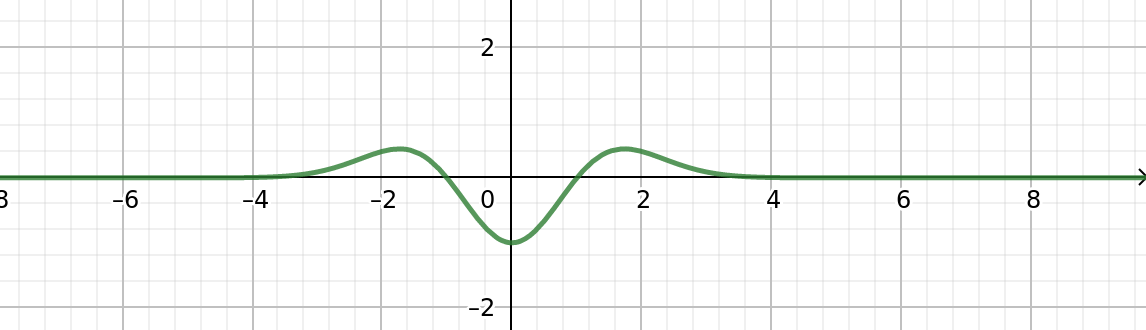
\includegraphics[scale=.4]{wykres_error.png}}
\caption{Wykres drugiej pochodnej (wygenerowany przez geogebra.org)}
\label{fig:error}
\end{figure}

Widać, że maksimum funkcji jest na pewno mniejsze niż 1, zatem funkcję błędu możemy oszacować przez ($N$ - liczba podprzedziałów, $a,b$ - krańce przedziału):
$$|E(N)| \leq \frac{(b-a)^3}{12N^2}$$
Pozostaje nam rozwiązać nierówność (względem N):
$$ \frac{(b-a)^3}{12N^2} \leq 10^{-8} $$
$$N \geq \sqrt{\frac{(b-a)^3 \cdot 10^{8}}{12}}$$
Zatem, wystarczy sprawdzić na wejściu programu, ile podprzedziałów potrzebujemy aby uzyskać zadaną dokładność. W przypadku metody Romberga (wiemy z Analizy Numerycznej że działa ona mniej więcej 2 razy lepiej) możemy podzielić na tyle samo podprzedziałów, aby mieć pewność, że metoda zwróci nam wynik z zadaną dokładnością. Na przykład dla $(b-a) = 1$, potrzebujemy $N \geq 10^4$ podprzedziałów.
\section{Program i wyniki eksperymentów}

Pełny program, który wykorzystuje wszystkie powyższe obserwacje znajduje się w pliku CDF\_standard\_ND.py. Oto kilka wyników eksperymentów:\\
Funkcja $I$ liczy wartość całki $I(a) = \int\limits_{0}^{a} \exp\left(-\frac{x^2}{2}\right)\,dx $, natomiast $\Phi$ liczy wartość dystrybuanty: $$\Phi(t) = \int\limits_{-\infty}^t f(x)\,dx = \int\limits_{-\infty}^t \frac{1}{\sqrt{2\cdot\pi}}\,\exp\left(-\frac{x^2}{2}\right)\,dx,\, t \in \mathbb{R}$$
Kilka wyników dla numerycznego liczenia wartości całki:
\begin{figure}[htbp]{}
\centerline{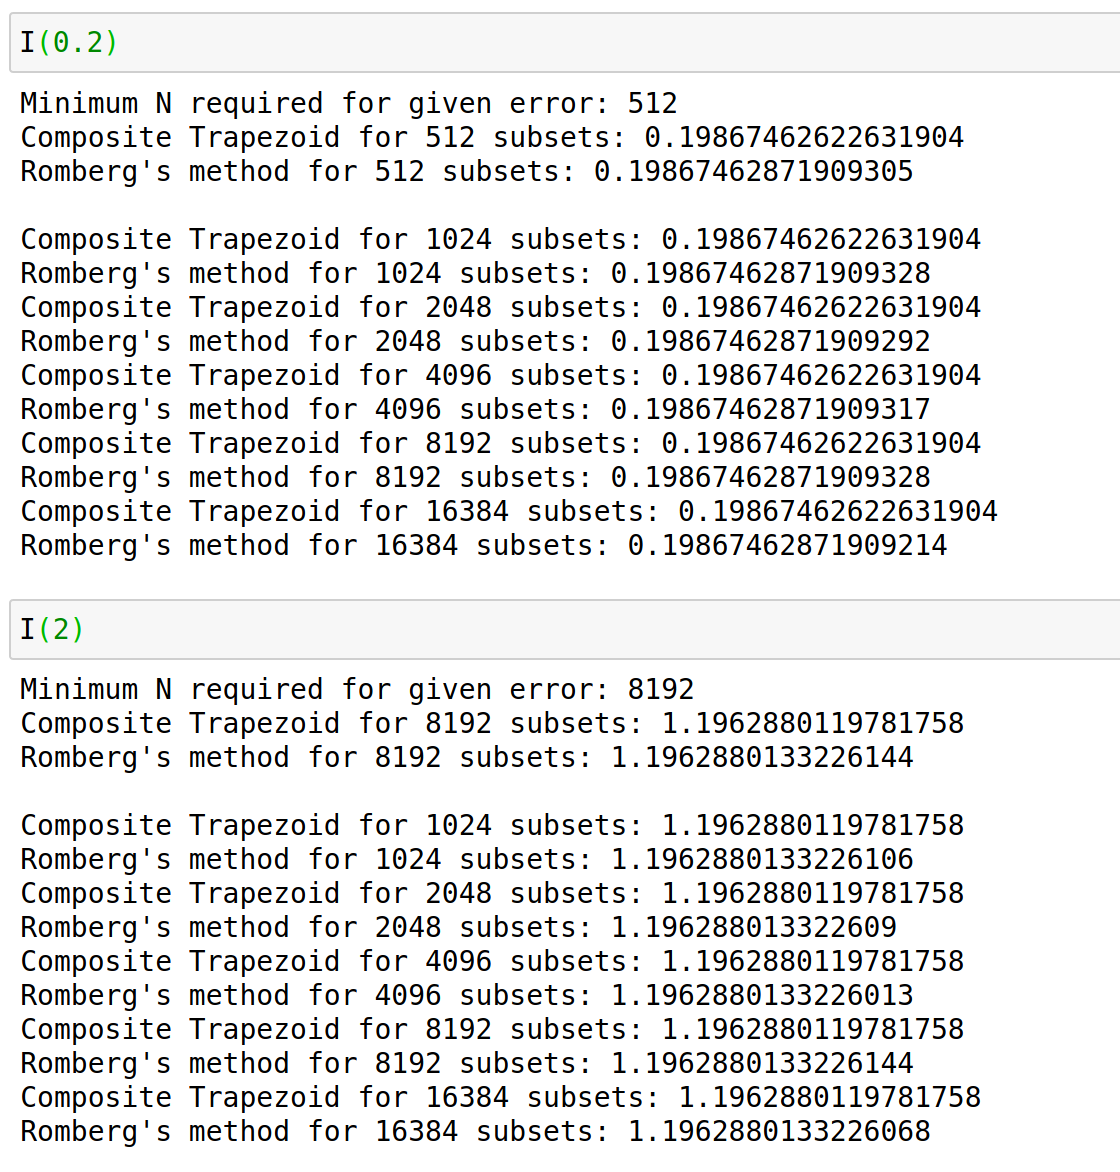
\includegraphics[scale=.25]{outputs_I.png}}
\label{fig:outputs_I}
\end{figure}

Możemy zauważyć, że metoda Romberga jest dokładniejsza i szybciej zbiega do dokładnego wyniku.


\newpage
Zaaplikujmy zatem metodę Romberga do wyliczenia naszej dystrybuanty:

\begin{figure}[htbp]{}
\centerline{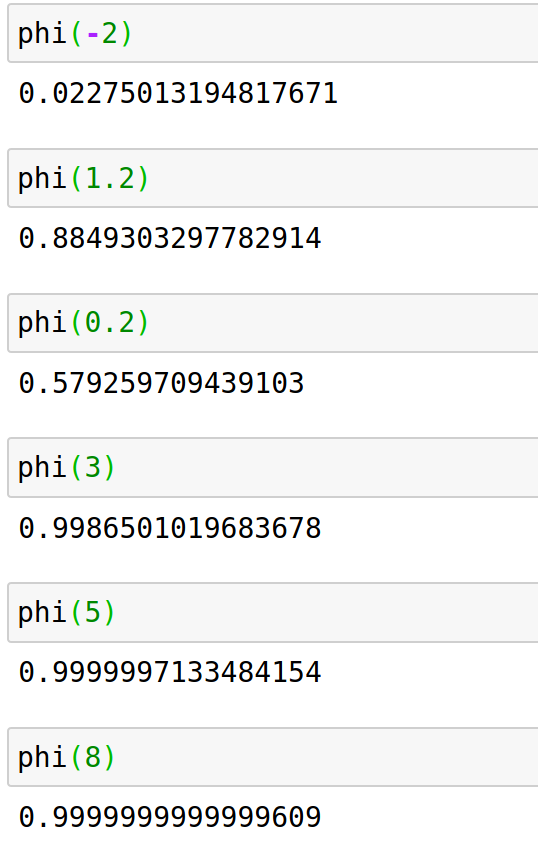
\includegraphics[scale=.30]{outputs_Phi.png}}
\label{fig:outputs_Phi}
\end{figure}

Zgodnie z oczekiwaniami wartości dystrybuanty oddalone o kilka sigm są coraz bliżej jedynki lub zera. Dodatkowo możemy sprawdzić, że wykres wygenerowany przez naszą dystrybuantę jest poprawny:

\begin{figure}[htbp]{}
\centerline{\includegraphics[scale=.1]{plot_Phi_wiki.png}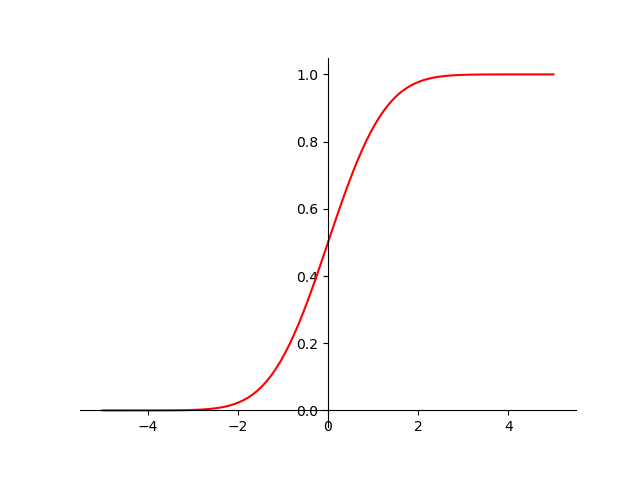
\includegraphics[scale=.5]{plot_Phi.png}}
\caption{Wykresy dystrybuanty rozkładu normalnego, po lewej widać wzorcowe wykresy z Wikipedii, po prawej wygenerowany przez nasz program dla funkcji Phi.}
\label{fig:plot_phi}
\end{figure}
\end{document}